\section{Aufgaben}

\subsection{hello-world.cc}
\begin{frame}{Ziel}
 \begin{itemize}
  \item \cod{hello-world} auf dem \host und auf dem \targetS
  \item \cod{primes} auf dem \host und auf dem \targetS
 \end{itemize}
\end{frame}


\begin{frame}{The big Picture}
 \begin{itemize}
  \item Source File: \cod{hello-world.cc}
  \item falls es nicht klapt ?
  \begin{itemize}
   \item wo ist der File ?
  \end{itemize}
 \end{itemize}
\end{frame}

\subsection{Zugriff auf die Hardware}
\begin{frame}{Scripts}
 \begin{itemize}
  \item \cod{led-enable.sh}
  \item \cod{led-blink.sh}
 \end{itemize}
\end{frame}

\begin{frame}{C++}{mit \cod{/sys/class/gpio}}
 \begin{itemize}
  \item \cod{led-enable.cc}
  \item \cod{led-blink.cc}
 \end{itemize}
\end{frame}

\begin{frame}{C++}{direkt mit \cod{mem.h$|$cc}}
 \begin{itemize}
  \item \cod{led-direct-0.cc}
  \item \cod{led-direct-1.cc}
 \end{itemize}
\end{frame}

\subsection{Zugriff auf die andere Hardware}

\begin{frame}{Input \& Output}
 \begin{center}
  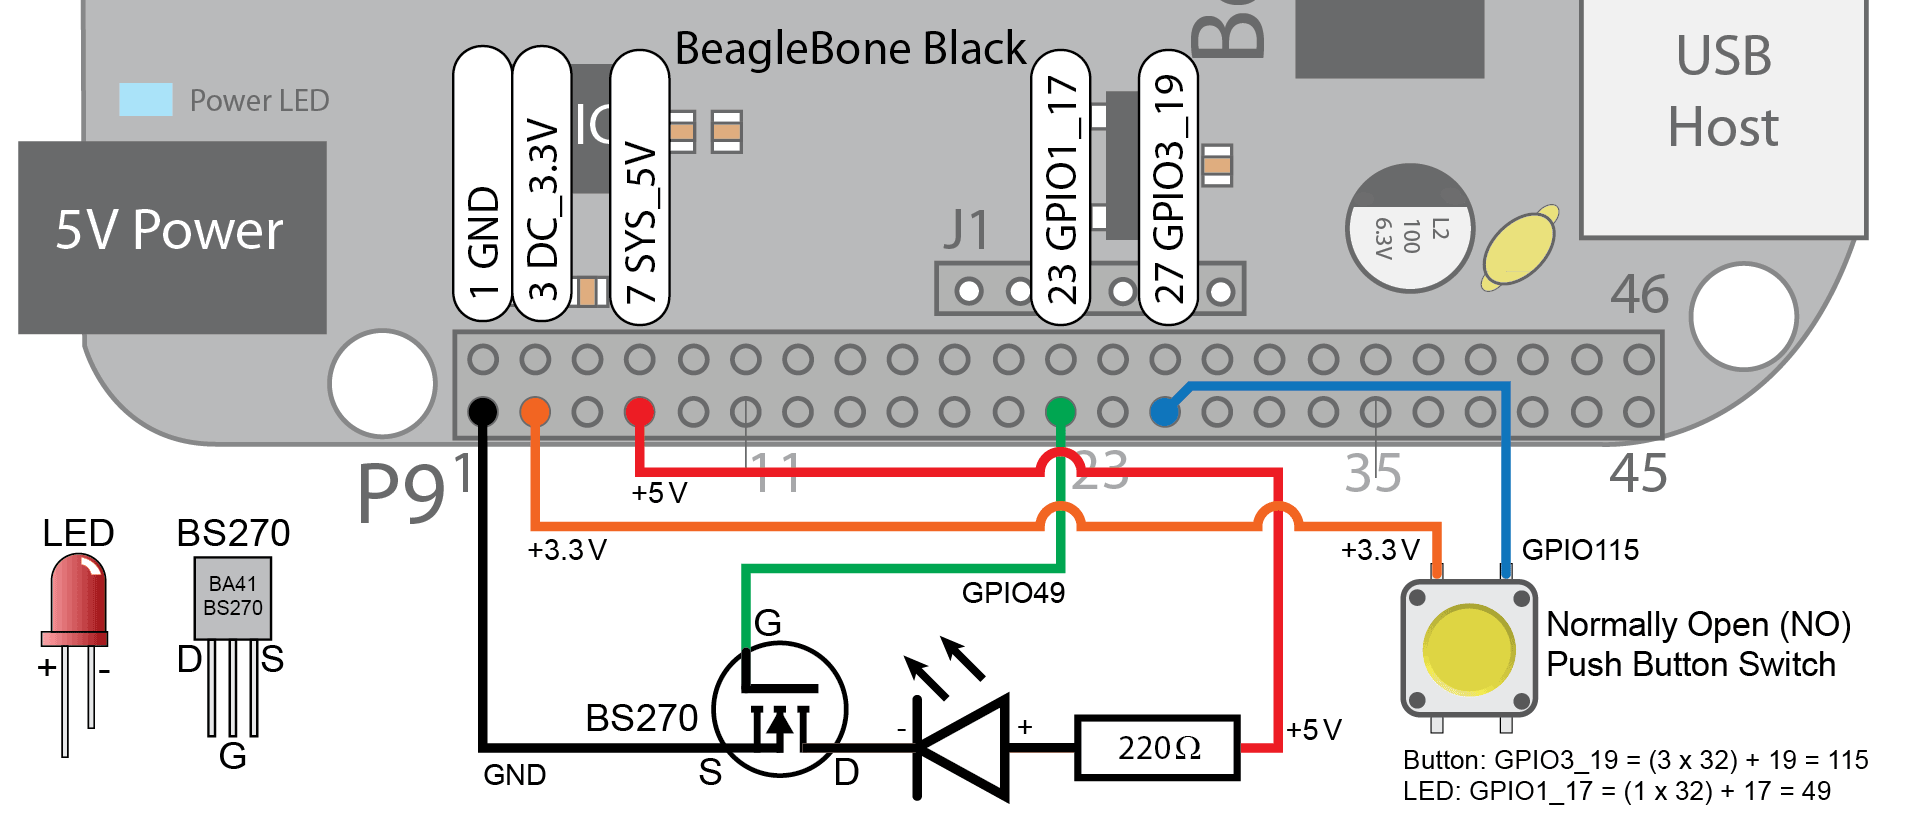
\includegraphics[width=0.875\textwidth]{Button-and-LED-large.png}
 \end{center}
 \begin{itemize}
  \item Output LED (Script,C++)
  \item Input SWITCH (Script,C++)
 \end{itemize}
\end{frame}

\begin{frame}{Input \& Output}{Kombination}
 \begin{itemize}
  \item SWITCH $\to$ LED
  \begin{itemize}
   \item Script
   \item C++
  \end{itemize}
 \end{itemize}
\end{frame}

%\subsection{Die Programme}
%\begin{frame}{Development}{\cod{hello-world-c.c}}
%\hspace*{-8mm}
%{
%\begin{tabular}{llllll}
% Host & Target & OS & Toolchain & Verbindung & Bemerkungen\\
% \hline
% \targetS & \targetS & Debian & mitgeliefert&&\\
% \host   & \targetS & Debian & \cod{\tiny tc-tinl-gcc-8.1.0-2018.05.21.tar.gz} & sshfs\\
% \host   & \targetS & minimal & \cod{\tiny tc-tinl-gcc-8.1.0-2018.05.21.tar.gz} & SD-Card  &später\\
% \host   & \targetS & minimal & \cod{\tiny tc-tinl-gcc-8.1.0-2018.05.21.tar.gz} & curlftpfs&später\\
%\end{tabular}
%}
%\remark{Toolchain auf der Cloud: \href{https://drive.switch.ch/index.php/s/A6H382zEGDrgfAL}
%       {\Huge tinL}}
%\end{frame}
